\medskip

Puisque l'on choisit une personne au hasard dans la population française, on est en situation d'équiprobabilité, et donc la loi uniforme permet d'assimiler les proportions à des probabilités.

\begin{enumerate}
	\item L'arbre représentant la situation est :

	\hfill~
	
	
	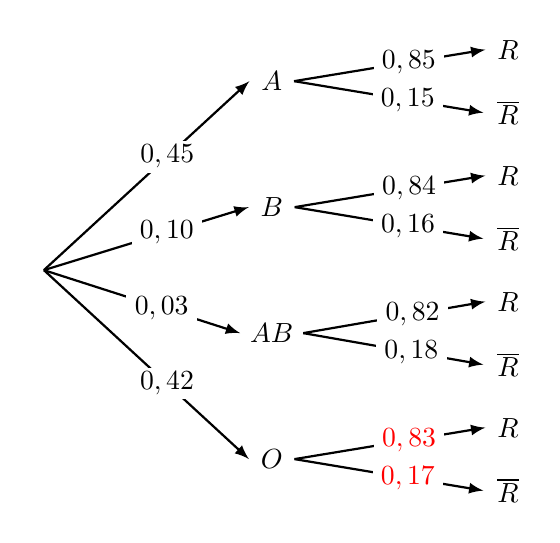
\begin{tikzpicture}[xscale=1,yscale=1,baseline={(R.base)}]
	
	\tikzstyle{fleche}=[->,>=latex,thick]
	\tikzstyle{noeud}=[fill=white,circle,inner sep=2pt]
	\tikzstyle{feuille}=[fill=white,circle,inner sep=2pt]
	\tikzstyle{etiquette}=[pos = 0.6,fill=white, inner xsep=3pt, inner ysep=1.5pt]
	
	\def\DistanceInterNiveaux{3}
	\def\DistanceInterFeuilles{0.8}
	
	\def\NiveauA{(0)*\DistanceInterNiveaux}
	\def\NiveauB{(1)*\DistanceInterNiveaux}
	\def\NiveauC{(2)*\DistanceInterNiveaux}
	\def\InterFeuilles{(-1)*\DistanceInterFeuilles}
	
	\node[noeud] (R) at ({\NiveauA},{(3.5)*\InterFeuilles}) {};
	\node[noeud] (Ra) at ({\NiveauB},{(0.5)*\InterFeuilles}) {$A$};
	\node[feuille] (Raa) at ({\NiveauC},{(0)*\InterFeuilles}) {$R$};
	\node[feuille] (Rab) at ({\NiveauC},{(1)*\InterFeuilles}) {$\overline{R}$};
	\node[noeud] (Rb) at ({\NiveauB},{(2.5)*\InterFeuilles}) {$B$};
	\node[feuille] (Rba) at ({\NiveauC},{(2)*\InterFeuilles}) {$R$};
	\node[feuille] (Rbb) at ({\NiveauC},{(3)*\InterFeuilles}) {$\overline{R}$};
	\node[noeud] (Rc) at ({\NiveauB},{(4.5)*\InterFeuilles}) {$AB$};
	\node[feuille] (Rca) at ({\NiveauC},{(4)*\InterFeuilles}) {$R$};
	\node[feuille] (Rcb) at ({\NiveauC},{(5)*\InterFeuilles}) {$\overline{R}$};
	\node[noeud] (Rd) at ({\NiveauB},{(6.5)*\InterFeuilles}) {$O$};
	\node[feuille] (Rda) at ({\NiveauC},{(6)*\InterFeuilles}) {$R$};
	\node[feuille] (Rdb) at ({\NiveauC},{(7)*\InterFeuilles}) {$\overline{R}$};
	
	\draw[fleche] (R.east)--(Ra.west) node[etiquette] {$0,45$};
	\draw[fleche] (Ra.east)--(Raa.west) node[etiquette] {$0,85$};
	\draw[fleche] (Ra.east)--(Rab.west) node[etiquette] {$0,15$};
	\draw[fleche] (R.east)--(Rb.west) node[etiquette] {$0,10$};
	\draw[fleche] (Rb.east)--(Rba.west) node[etiquette] {$0,84$};
	\draw[fleche] (Rb.east)--(Rbb.west) node[etiquette] {$0,16$};
	\draw[fleche] (R.east)--(Rc.west) node[etiquette] {$0,03$};
	\draw[fleche] (Rc.east)--(Rca.west) node[etiquette] {$0,82$};
	\draw[fleche] (Rc.east)--(Rcb.west) node[etiquette] {$0,18$};
	\draw[fleche] (R.east)--(Rd.west) node[etiquette] {$0,42$};
	\draw[fleche] (Rd.east)--(Rda.west) node[etiquette,text=red] {$0,83$};
	\draw[fleche] (Rd.east)--(Rdb.west) node[etiquette,text=red] {$0,17$};
	\end{tikzpicture}
	\hfill~

\emph{Remarque :} les deux probabilités en rouge n'étaient pas attendues ici. On peut compléter ces deux branches après avoir répondu à la question \textbf{3.}

\item  $P(B \cap R)=P(B) \times P_B(R)= 0,10 \times 0,84=0,084$.

Dans le contexte de l'exercice, $8,4\%$ de la population est de groupe sanguin B et de rhésus positif.

\item   Les évènements $A$, $B$, $AB$  et $O$ forment une partition de l'univers, donc, d'après la formule des probabilités totales :

\quad $P(R) = P\big(\,A\cap R\big) + P\big(\,B\cap R\big) +  P\big(\,AB\cap R\big) +P\big(\,O\cap R\big) $

D'où :\quad 
$\begin{aligned}[t] P\big(\,O\cap R\big)&  = P(R)  -P\big(\,A\cap R\big) - P\big(\,B\cap R\big) -  P\big(\,AB\cap R\big) \\
	&= \np{0,8397} - 0,45\times 0,85 - 0,084 - 0,03 \times 0,82\\
	& = \np{0,3486}
\end{aligned}$

Or $P_O(R)=\dfrac{P(O\cap R) }{P(O)}= \dfrac{\np{0,3486}}{0,42}= 0,83$

Ce qui est le résultat donné.

\item Trouver  la probabilité qu'un individu choisi au hasard dans la population française soit donneur universel  revient à calculer la probabilité  $P\left( O\cap \overline{R} \right)$.

$\begin{aligned} P\left( O\cap \overline{R} \right)& = P(O)\times P_{O}\left(\overline{R}\right)\\
	&= P(O)\times \left(1- P_{O}(R)\right)\\
	&= 0,42 \times (1 - 0,83)\\
	&= 0,0714
\end{aligned}$

La probabilité d'être un donneur universel est bien  de $\np{0,0714}$.

\item
	\begin{enumerate}
		\item  On répète 100 fois de manière identique et indépendante une expérience aléatoire à deux issues dont le succès \og la personne est un donneur universel\fg{}  a une probabilité $p=0,0714$.

La variable aléatoire $X$ compte le nombre de succès.

Donc $X$ suit une loi binomiale de paramètres $n=100$ et $p=\np{0,0714}$.
		\item $P(X \leq 7 ) \approx \np{0,57714}$.

À $10^{-3}$ près, la probabilité  qu'il y ait au plus 7 donneurs universels dans cet échantillon vaut $0,577$.
		\item  $X$ suit une loi binomiale de paramètres $n=100$ et $p=\np{0,0714}$ donc :

$\begin{aligned}[t] E(X)& =n \times p \\&= 100 \times 0,0714\\&=7,14\end{aligned}$
	\hfill~
$\begin{aligned}[t] V(X)& = n \times p \times (1-p)\\& = 100 \times 0,0714 \times (1- 0,714) \\& = \np{6,630204}\\
	& 	\approx 6,63\quad\text{ à }10^{-2} \text{ près.}
\end{aligned}$
\hfill~
	\end{enumerate}
\item
	
	
	
	
	
	\begin{enumerate}
		\item  La variable aléatoire $M_{N}$ dans le contexte de l'exercice représente le nombre moyen de donneurs universels sur les $N$ collectes de sang organisées.

		\item  $M_N$ est la moyenne empirique de la variable aléatoire $X$ donc :
		
$E\left(M_{N}\right)=E(X) =7,14$.
		\item

$V\left(M_{N}\right)=\dfrac{V(X)}{N}= \dfrac{6,63}{N}$.
		\item L'évènement \quad $\big\{ 7<M_{N}<7,28 \big\}$\quad revient à \quad $\big\{\big|M_{N} - 7,14\big| < 0,14\big\}$

et \quad $P\Big(\big|M_N - 7,14 \big| < 0,14\Big) = 1 - P\Big(\big|M_{N} - 7,14 \big| \geqslant 0,14\Big)$.

On veut que $P\Big(\big|M_{N} - 7,14 \big| \geqslant 0,14\Big) \geqslant 0,95$

On veut donc que $P\Big(\big|M_N - 7,14 \big| < 0,14\Big) \leqslant 0,05$

Or, pour tout réel $t > 0$, d'après l'inégalité de Bienaymé-Tchebychev, on a :

$P\Big(\big|M_N-E\big(\,M_N\big)\big| \geqslant t\Big) \leqslant \dfrac{V\big(\,M_N\big)}{t^2}$

Pour $t = 0,14$ on obtient : $ P\Big(\big|M_N-7,14\big| \geqslant 0,14\Big)\leqslant \dfrac{6,63}{ N \times 0,14^2}$.

On veut donc que :\quad $\begin{aligned}[t]
	\dfrac{16575}{49 N} \leqslant 0,05 &\iff
	\dfrac{331500}{49} \leqslant N \\
	&\iff 6765+\dfrac{15}{49}\leqslant N
\end{aligned}$

L'inégalité est donc vraie pour tout entier $N \geqslant \np{6766}$.

La plus petite valeur de $N$ pour laquelle l'inégalité de Bienaymé-Tchebychev permet d'affirmer que $P\left(7<M_{N}<7,28\right) \geqslant 0,95$ est $\np{6766}$.

	\end{enumerate}
\end{enumerate}

\bigskip
